\documentclass[a4paper]{article}
\usepackage[T1]{fontenc}
\usepackage[utf8]{inputenc}
\usepackage{lmodern}
\usepackage{graphicx}
\usepackage[left=2.5cm,right=2.5cm,top=3cm,bottom=3cm]{geometry}
\usepackage{eurosym}
\usepackage{fancyhdr}%encabezado y pie de página
\usepackage[colorlinks=true, linkcolor=black, urlcolor=blue]{hyperref}
\setcounter{secnumdepth}{5}
\usepackage[spanish]{babel}
\setcounter{tocdepth}{5}
\usepackage{colortbl}%para colorear tablas
\usepackage{tabularx}
\usepackage{placeins}%para poner barrera y no pasen de secciones los elementos flotantes
%\usepackage{wasysym} %para poner símbolos
\usepackage{bbding} %para poner símbolos



%para el mapa mental
\usepackage{tikz}
\usetikzlibrary{mindmap,trees}
\usepackage{verbatim}


\date{}
\author{D. Ramirez Ambrosi \\ J. I. Sánchez Méndez \\ J. Rodríguez Azpeleta}
\title{\begin{center}
\textbf{\Huge{Make Yourself Strong}} \\ Evaluación de prototipos  \\Proyecto de la asignatura Interacción Persona Computador \\ \Huge{Grupo 10}
\end{center}}
\date{\today}


\pagestyle{fancy}
\rhead{
\textbf{Make Yourself Strong} \hfill \textbf{Fecha:} \date{\today}
}

\lhead{}

%Separación entre párrafos
\setlength{\parskip}{3mm}

%colores
\definecolor{verde}{RGB}{127,255,0}%color para la barra de titulo
\definecolor{rojo}{RGB}{255,0,0}%color para características
\renewcommand\listfigurename{\centering LISTA DE FIGURAS}

\begin{document}
\maketitle

\thispagestyle{empty}%para evitar enumeración de la página de la portada y del índice
\newpage
\tableofcontents%índice
\thispagestyle{empty}
\newpage



%lista de figuras 
%\renewcommand\listfigurename{\centering LISTA DE FIGURAS}
%\listoffigures
%\clearpage

%Lista de tablas
%\renewcommand{\listtablename}{\centering ÍNDICE DE TABLAS} %Para cambiar el índice de las tablas
%\listoftables
%\thispagestyle{empty}
%\newpage

\setcounter{page}{1}%Para reiniciar el contador de páginas en la página deseada


\section{Resultados de la evaluación}

\subsection{Desglose por categorías}

\begin{figure}[!h]
\centering
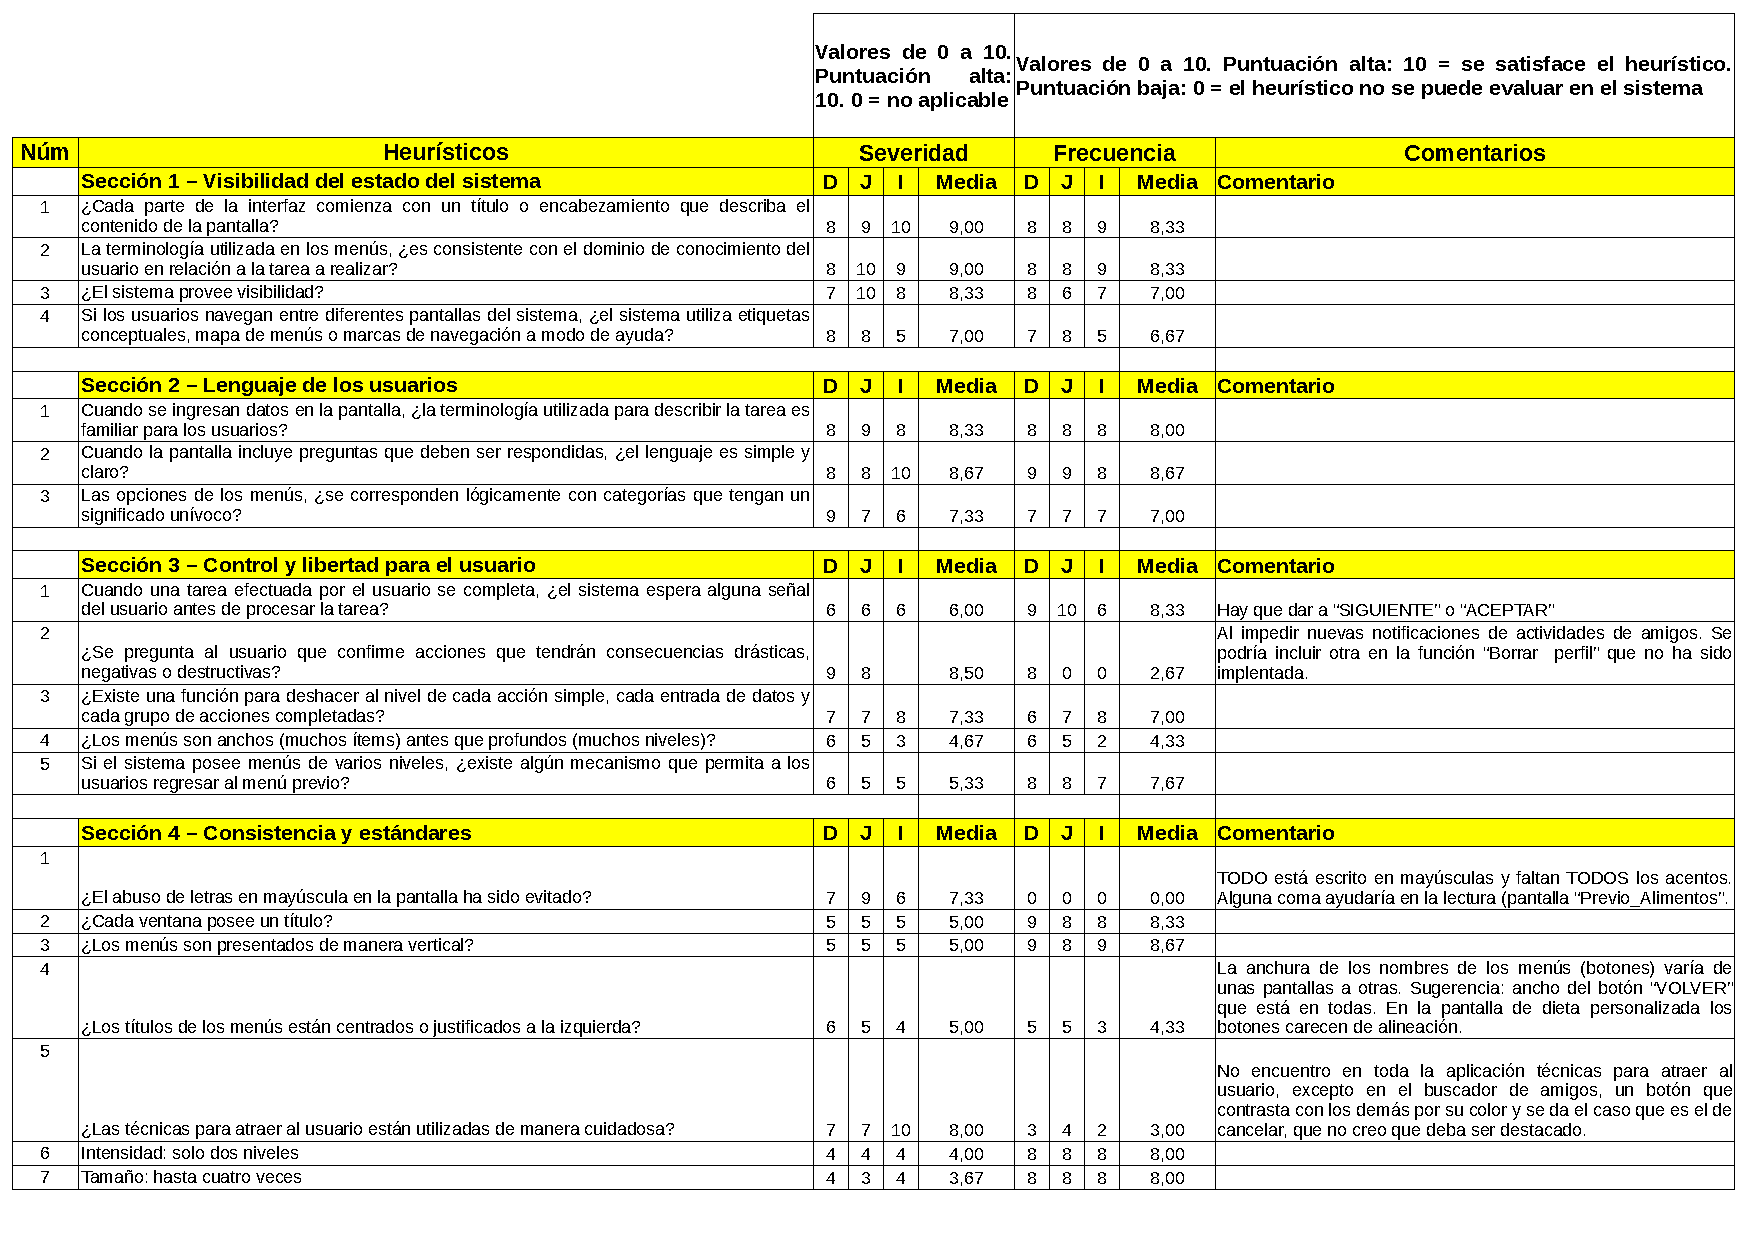
\includegraphics[width=0.9\textheight,angle=90,page=1]{./figuras/checklist.pdf}
\end{figure}

\begin{figure}[!h]
\centering
\includegraphics[width=0.9\textheight,angle=90,page=2,clip=true,trim=0 3cm 0 0]{./figuras/checklist.pdf}
\end{figure}

\begin{figure}[!h]
\centering
\includegraphics[width=0.9\textheight,angle=90,page=3,clip=true,trim=0 14cm 0 0]{./figuras/checklist.pdf}
\end{figure}
\FloatBarrier

\subsection{Resumen resultados}

\begin{figure}[!h]
\centering
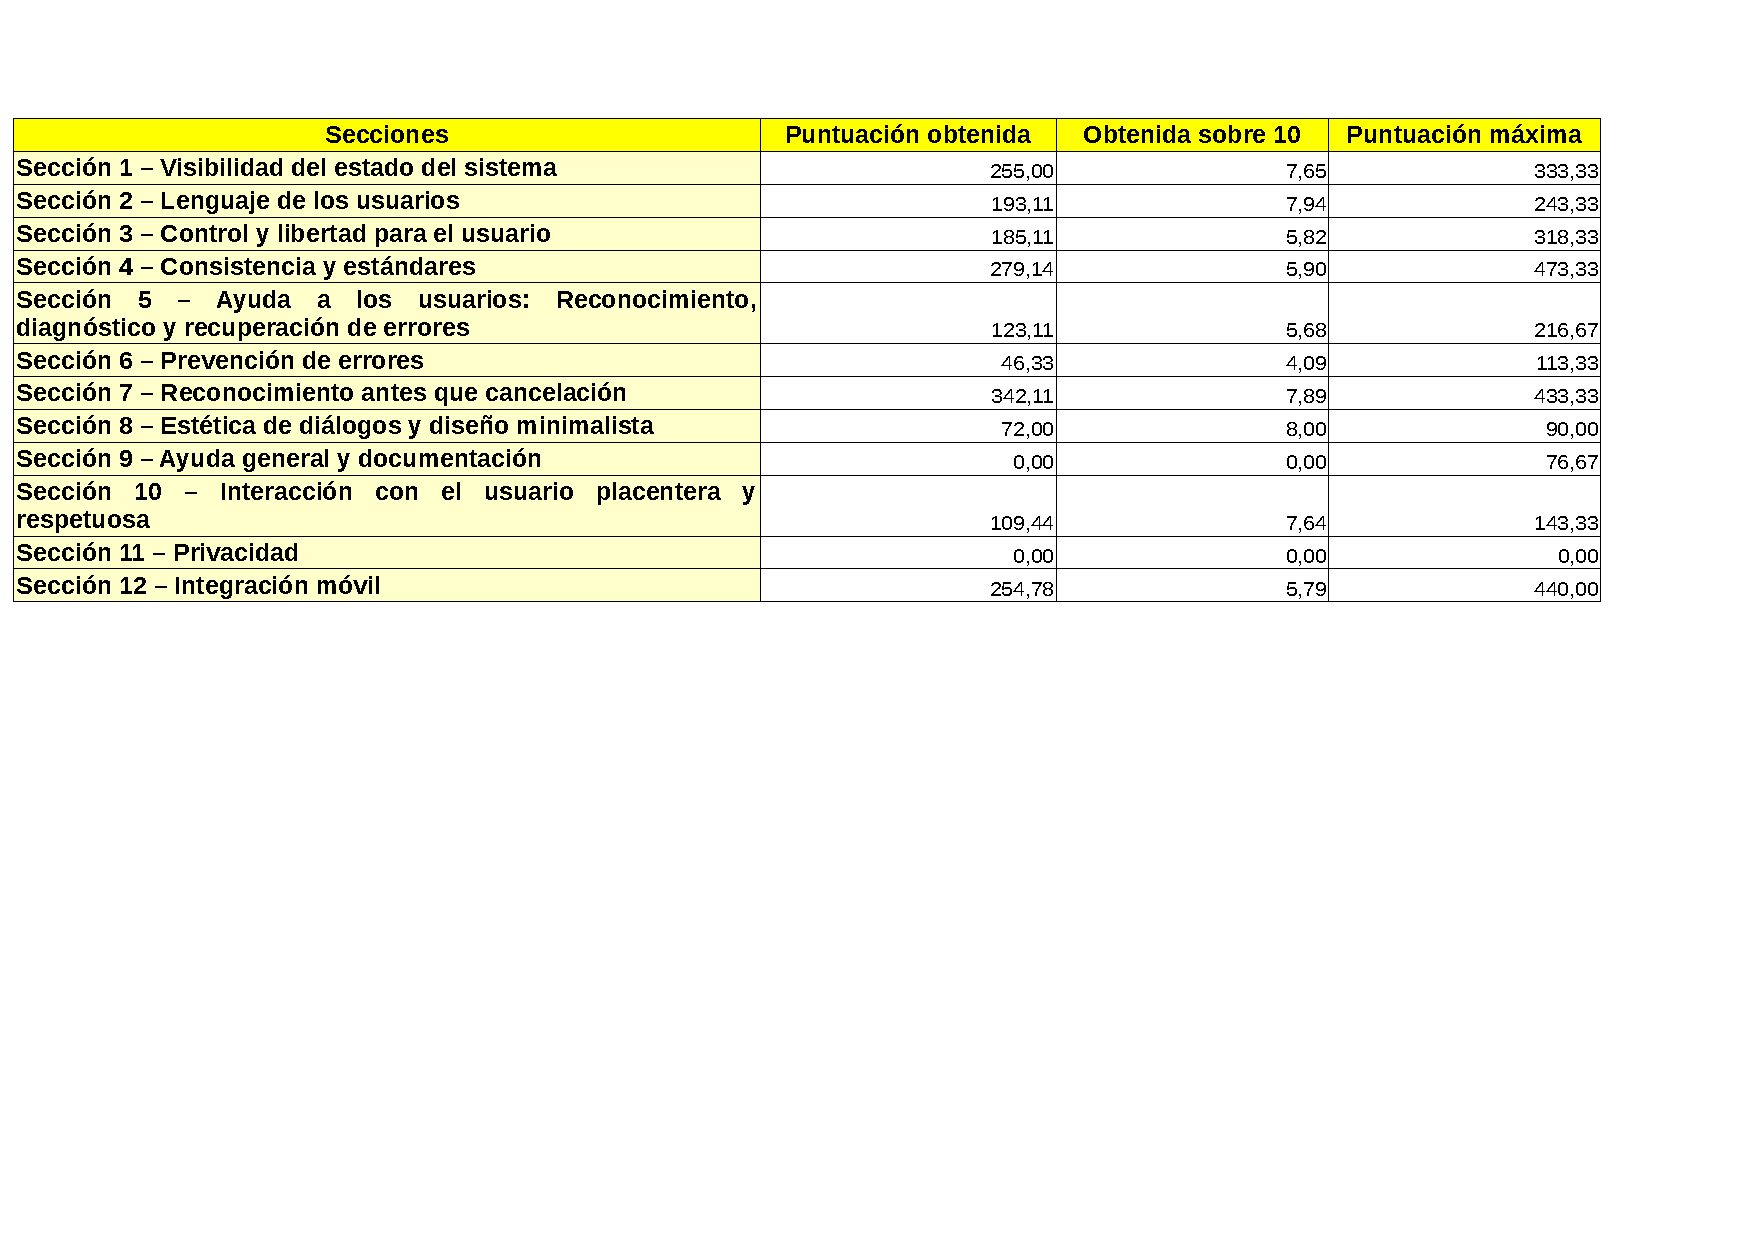
\includegraphics[width=0.9\textheight,angle=90,clip=true,trim=0 10cm 0 0]{./figuras/resultados.pdf}
\caption{Resumen evaluación}
\end{figure}
\FloatBarrier

\section{Valoraciones personales}

\subsection{Josu Rodríguez}

Los textos y sus formatos podrían estar más cuidados, el uso de mayúsculas es excesivo y en varias ocasiones el tamaño de letra puede ser un poco pequeño.

Algunos botones difieren de tamaño entre sí en las mismas ventanas lo que resta algo de coherencia. Además, varios textos de los botones son más grandes que los mismos por lo que no se ven en su totalidad.

Hay algún fallo puntual como que las pulsaciones no se miden en pulsaciones por minuto, la medida es incorrecta. 

La interacción me ha gustado y la navegación a través de los menús resulta intuitiva. En general está bien adaptado a una interfaz móvil y parecería bastante usable si se llevase a cabo.

\subsection{Jose Ignacio Sánchez}

La tecnología móvil ofrece más posibilidades para facilitar la navegación, como
menús de cada frame que puede guardar las configuraciones genéricas o incluso
menús laterales ocultables que permiten una navegación más rápida entre las
distintas pantallas, aunque la navegación es intuitiva y usable.

En general está bien adaptado y utilizan una temática adecuada, aunque yo
profundizaría un poco más en uno de los dos aspectos(dietética o entrenamiento),
para poder ofrecer algo más personalizado como un contacto entre nutricionistas
y usuarios.


\subsection{David Ramirez}

Algún pequeño detalle que he encontrado: al cancelar la búsqueda de amigos se vuelve al menú ``Ejercicios para hoy'' en el prototipo verde. En el azul está corregido pero en menú tiene una errata "BUSCRA AMIGOS".

Un tema a mejorar son los textos. Todos están escritos con mayúsculas y carecen de acentos, además de alguna falta de redacción. Por ejemplo, en la pantalla de búsqueda de amigos ``RELLENA ALGUN DE LOS CAMPOS'' o la nota ``Previo\_ejercicio'' en ambos prototipos.

En cuanto a su visualización, es correcta en general. Un caso particular es la nota que se muestra antes de seleccionar las preferencias con letras blancas sobre fondo gris. En el prototipo azul, las letras blancas sobre el fondo azul se distinguen mejor.

A la hora de elegir los alimentos que le gustan al usuario para la configuración de la dieta, los elementos que se despliegan de las diferentes secciones no se distinguen de la sección. En ambos prototipos poseen el mismo color. Además, todos los elementos están pulsados por defecto, sería mejor que no lo estuvieran, de esa forma el usuario podría seleccionar los que le interesaran. De esta forma, cada semana podría seleccionar los alimentos que quisiera de forma más rápida y sería más fácil variar de alimentos, por ejemplo.

En la sección de estadísticas solo se muestran las correspondientes a correr. En nuestra página también pusimos una única imagen, pero sería mejor que hubiese un menú que muestre que en la aplicación habrá más tipos de estadísticas como evolución de peso, de calorías ingeridas, de otros entrenamientos...

En cuanto a la sección de ejercicios. Comenzando por la tabla de ejercicios, estaría bien que se pudiera cambiar el número de saltos, por ejemplo. Durante el entrenamiento, pantalla ``Ejercicio'' tengo la sensación de que las pulsaciones se miden en minutos tal y como está puesto, sugiero: ``Pulsaciones: 85 /min''. También hay que cuidar más la longitud del texto de los botones en esta pantalla.

En la sección de ejercicio específico, sugiero usar como títulos o bien el nombre del músculo o grupo de músculos, o la parte del cuerpo que se trabaja, pero no mezclarlos. Pondría: Hombro, BRAZO, PECHO, Abdomen, ESPALDA, Pierna para dar mayor uniformidad.

En la sección de Correr no me cuadra que tras seleccionar un tiempo y sin seleccionar una ruta, la pantalla de estado sea de una ruta concreta.

En cuanto a las Rutas Sugeridas, se muestran los diferentes niveles que son desplegables, el espacio de color no se aprovecha para nada. Sugiero cambiar a dos desplegables. En el primero se selecciona el nivel. Con éste seleccionado, se habilita el segundo con las rutas correspondientes cargadas. Se selecciona la ruta y se pulsa correr.

En general la interacción me ha parecido que estaba bastante bien, aunque al pasar de leer algunos mensajes, luego no se sabe qué hacer en la pantalla siguiente.

\section{Valoración grupal}

Coincidimos en que la interfaz resulta usable y la navegación a través de los menús resulta intuitiva. Explotando las capacidades de las APIS de programación se podría mejorar el aprovechamiento del espacio en la pantalla. Por ejemplo, deslizar hacia la derecha para que aparezca el menú en vez del botón en la pantalla, aunque también entendemos las limitaciones de los sistemas de prototipado.

En general cabe destacar la corrección del abuso de las letras mayúsculas y las faltas ortográficas en la aplicación, así como algún error conceptual ya mencionado (pulsaciones por minuto). Otros pequeños detalles son el alineamiento de los  botones así como su tamaño y el del texto contenido en los mismos.

En cuanto a funcionalidad, es abundante y cualquier usuario interesado en este tipo de aplicación sabrá sacarle provecho. No obstante, si que corregiríamos algunas interacciones de la aplicación como la de selección de rutas para salir a correr y la de selección de alimentos preferentes para la dieta.
 
\end{document}
